\subsection*{Report 2}

	In the second exercise we simulated sound travelling from a source to a target, with first and second order reflections from the walls being included. The MATLAB script used can be found on page \pageref{matlab_1.2}. A damping factor of 0.5 is used to allow the signals to decrease over time, as they would in reality. An impulse response was sent as the source, and from the simulated received pulses, we also calculated the room channel impulse response through a convolution of the original impulse response and the simulated received response. Below in figure \ref{figure:1_2} we can see that both the received signal and calculated response are the same, as expected.
	
	\begin{figure}[H] 
		\centering
		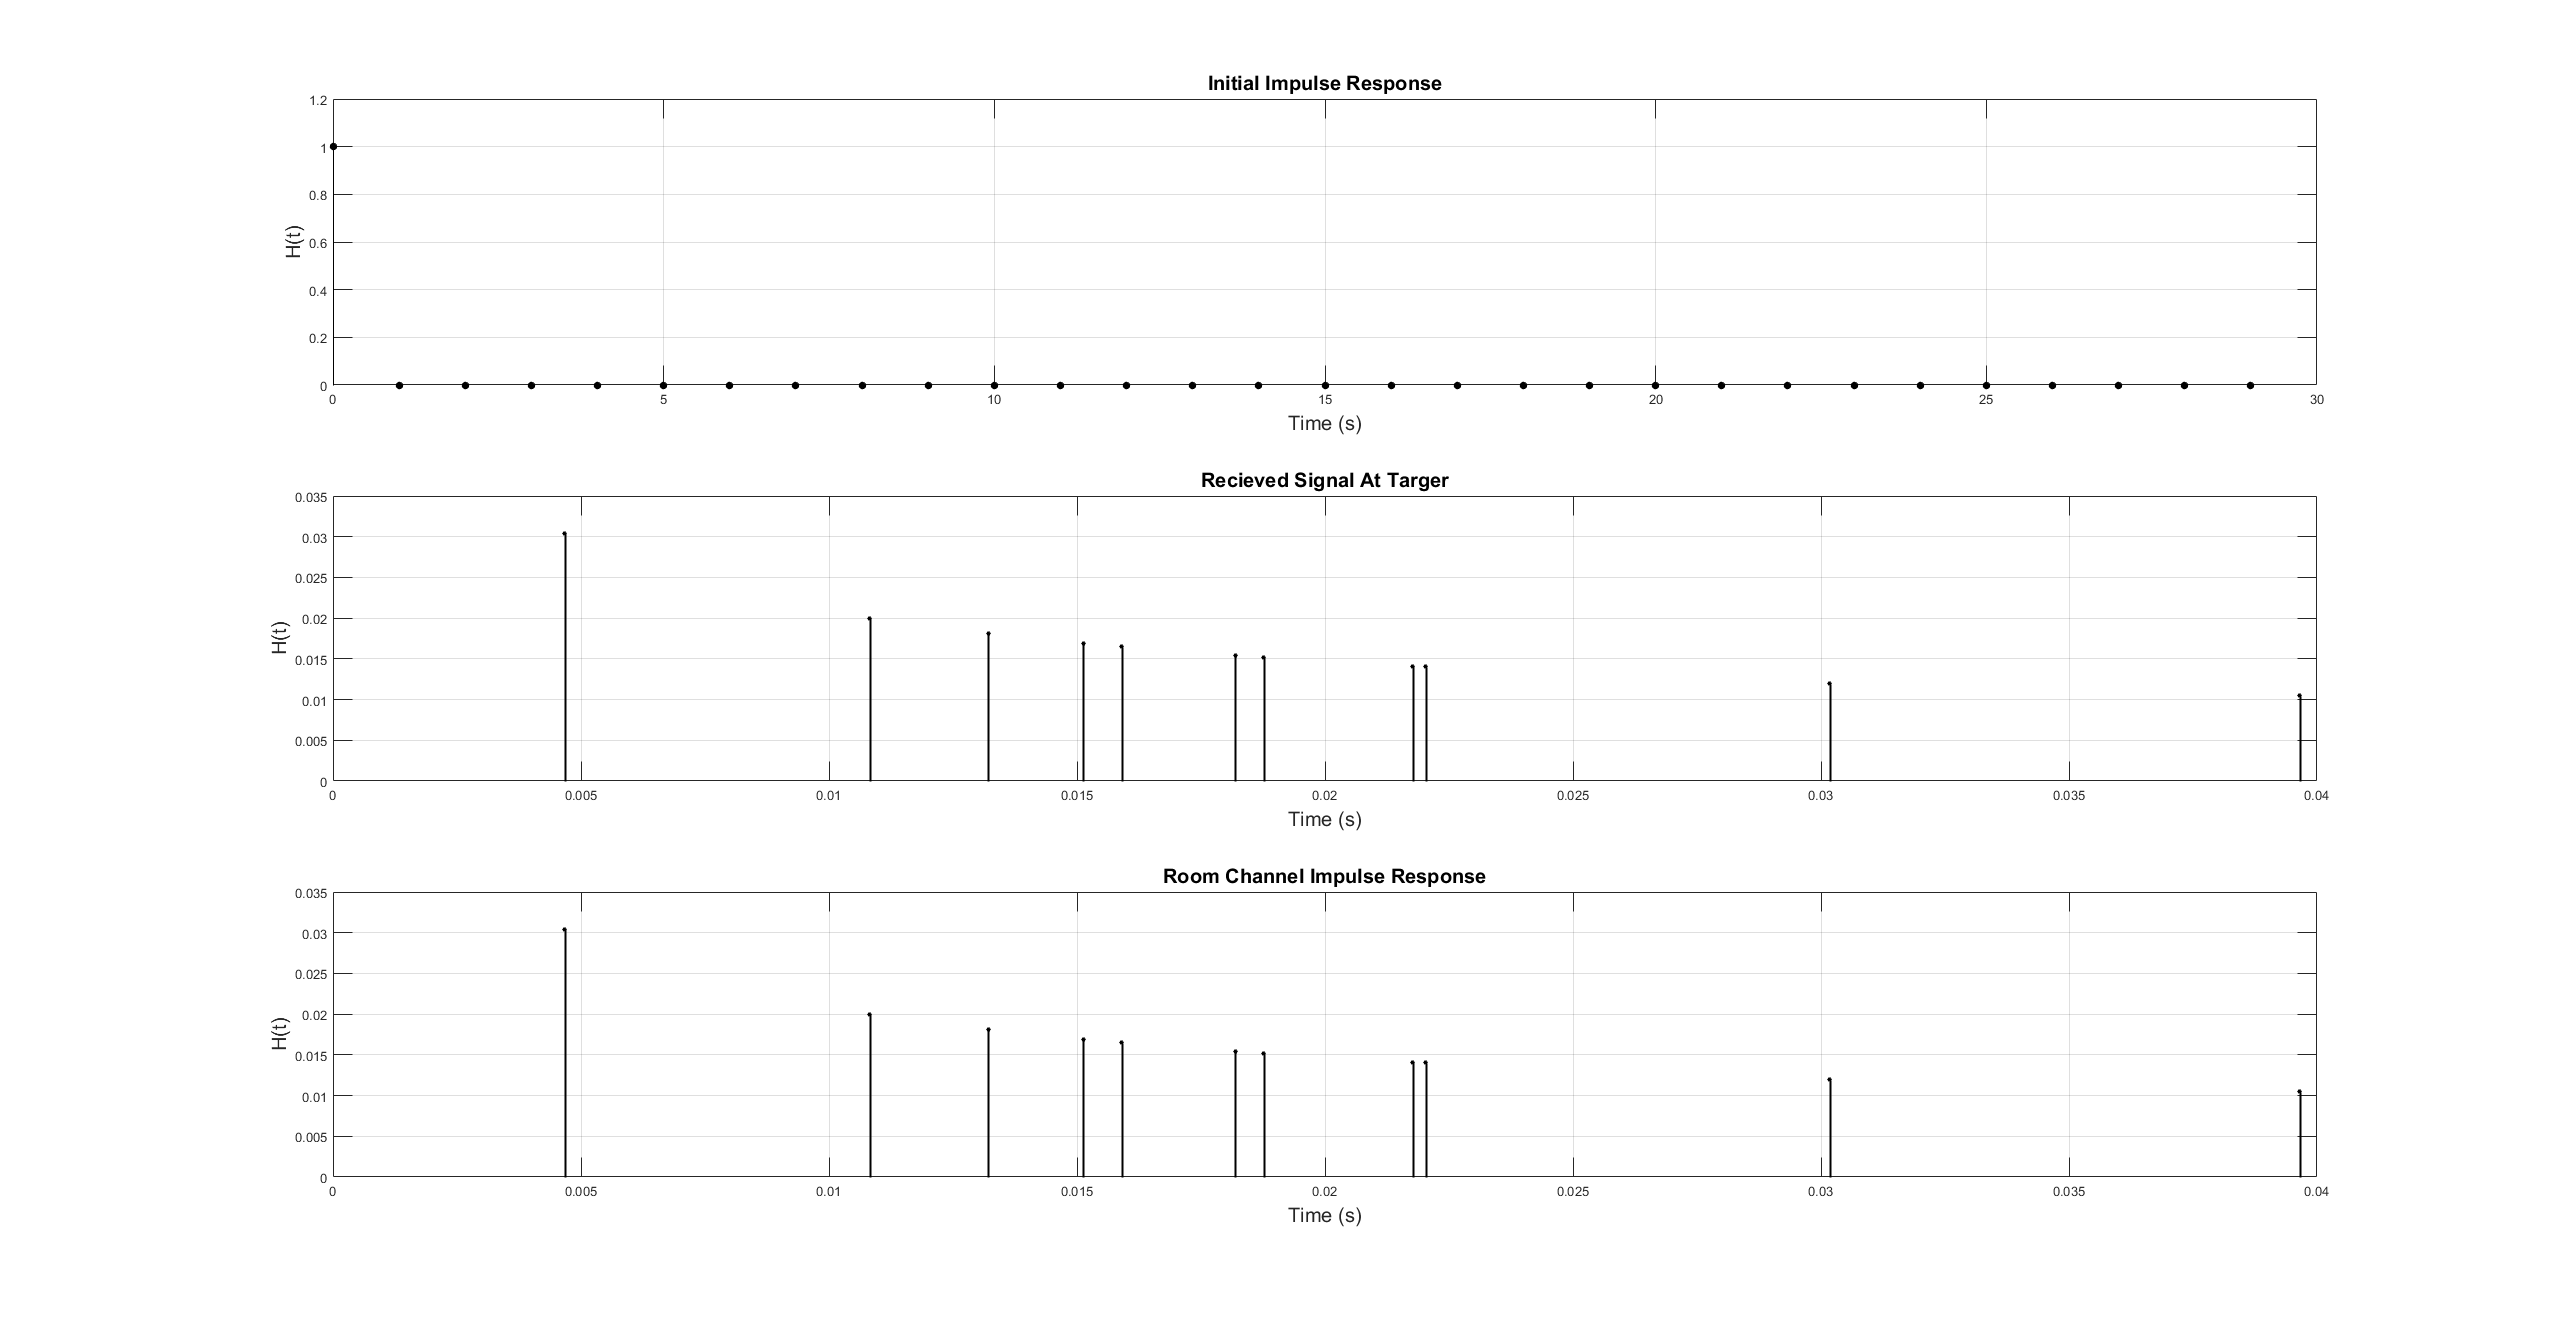
\includegraphics[width=\textwidth]{1.2.png}
		\caption{Room Channel Impulse Response \& Reflected Signals}
		\label{figure:1_2}
	\end{figure}